\message{ !name(rfsm.tex)}\documentclass[a4paper]{report}

\usepackage{amsmath,amssymb,stmaryrd,latexsym}
\usepackage{titlepic}
\usepackage{syntax}
\usepackage{multicol}
\usepackage{alltt}
\usepackage{graphicx}   % Including Graphics
%\usepackage{verbatim} 
\usepackage{spverbatim}
\usepackage{alltt} 
\usepackage{xspace} 
\usepackage{listings} 
\usepackage{ifthen}
\usepackage{adjustbox}
\usepackage{xhfill}% http://ctan.org/pkg/xhfill
\usepackage{color}
\usepackage{fancybox}
\usepackage{fancyvrb}
\usepackage{fixltx2e}
\usepackage[multiple]{footmisc}
\usepackage{grammar-defns}  %% Generated by Obelisk
\usepackage{url}

\newsavebox{\FVerbBox}
\newenvironment{FVerbatim}
 {\VerbatimEnvironment
  \begin{center}
  \begin{lrbox}{\FVerbBox}
  \begin{BVerbatim}}
 {\end{BVerbatim}
  \end{lrbox}
  \fbox{\usebox{\FVerbBox}}
  \end{center}}

\newboolean{devel}
\setboolean{devel}{false}

\lstloadlanguages{C++,VHDL}
\lstset{frameround=tttt} 
\lstset{captionpos=t}
\lstset{breaklines=true}
\lstset{escapechar=@}
%\lstset{aboveskip=2\medskipamount}
%\lstset{belowskip=1.5\medskipamount}
%\lstset{abovecaptionskip=\medskipamount}
\lstdefinelanguage{Rfsm}{keywords={type,enum,record,function,return,fsm,model,in,out,inout,vars,states,trans,itrans,on,when,with,periodic,sporadic,value_changes,event,bool,input,output,shared,where,and},morecomment=[l]{--}}
\lstdefinelanguage{ctask}{language=C,morekeywords={task,wait_ev,wait_evs,notify_ev,in,out,inout}}
\lstdefinelanguage{systemc}{language=C++,morekeywords={SC_MODULE,SC_METHOD,SC_THREAD,sc_in,sc_out,sc_inout}}

%%% Better hyphenation:
%\sloppy
\setlength{\topmargin}{0pt}
\setlength{\oddsidemargin}{0pt}
\setlength{\textheight}{600pt}
\setlength{\textwidth}{448pt}

%\Newcommand{\docdate}{\today} %%%!!!!
\newcommand{\step}{\medskip$\blacktriangleright$\xspace}

\newcommand{\version}{2.0}

\newcommand{\ie}{\emph{i.e.}\xspace}
\newcommand{\txt}[1]{\hbox{#1}}
\newcommand{\emtxt}[1]{\hbox{\em{#1}}}
\newcommand{\bftxt}[1]{\hbox{\bf{#1}}}
\ifthenelse{\boolean{devel}}{\newcommand{\note}[1]{\marginpar{\tiny #1}}}{\newcommand{\note}[1]{}}
\newcommand{\todo}[1]{\note{TODO: #1}}
\ifthenelse{\boolean{devel}}{\newcommand{\tbw}[1]{$\spadesuit$ {\bf To be written\ldots}\xspace}}{\newcommand{\tbw}[1]{}}
\ifthenelse{\boolean{devel}}{\newcommand{\tbc}[1]{$\spadesuit$ {\bf To be continued\ldots}\xspace}}{\newcommand{\tbc}[1]{}}

\newcommand{\rfsm}{RFSM\xspace}
\newcommand{\ocaml}{{\sc Objective Caml}\xspace}

\newcommand{\example}[1]{\fcolorbox{white}{lightgray}{#1}}
\newcommand{\ifname}[3]{$\mathtt{#1}_{\mathtt{#2}}\mathtt{#3}$}

%\newenvironment{example}{\medskip\noindent{\it Example :}\begin{alltt}}{\end{alltt}}

\title{RFSM User Manual - \version}

\author{J. S\'erot}

\titlepic{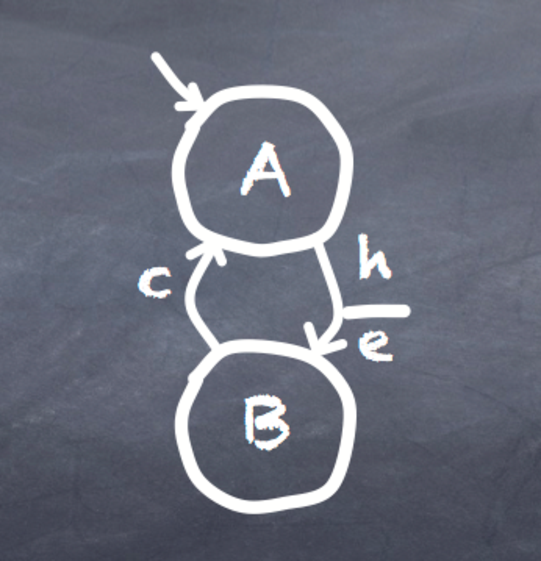
\includegraphics[width=0.5\textwidth]{figs/rfsm-logo}}
\date{}

\begin{document}

\message{ !name(introduction.tex) !offset(-89) }
\chapter{Introduction}
\label{chap:intro}

This document is a brief user manual for the RFSM language and compiler. It is, in its current form, very
preliminary, but should suffice for a quick grasp of the language possibilities. 

\medskip
RFSM is a domain specific language aimed at describing, drawing and simulating \emph{reactive finite state
  machines}. Reactive FSMs are a FSMs for which transitions can only take place at the occurence of
events.

\medskip
RFSM has been developed mainly for pedagogical purposes, in order to initiate students to
model-based design. It is currently used in courses dedicated to embedded system design both on
software and hardware platforms (microcontrolers and FPGA resp.). But RFSM can also be used to
generate code (C, SystemC or VHDL) from high-level models to be integrated to existing applications.

More precisely, RFSM can be used to
\begin{itemize}
\item describe FSM-based models and testbenches,
\item generate graphical representations of these models (\verb|.dot| format) for visualisation,
\item simulate these models, producing \verb|.vcd| files to be displayed with waveform viewers such
  as \texttt{gtkwave},
\item generate C, SystemC and VHDL implementations (including testbenches for simulation)
\end{itemize}

\medskip
The RFSM compiler is also used internally by the \textsc{RfsmLight}
application\footnote{\url{github.com/jserot/rfsm-light}} which provides a GUI-based interface to a
subset of the language\footnote{Single FSM models only.} and compiler back-ends. The
\textsc{RfsmLight} application is described in a separate document.

\medskip
This document is organized as follows.
Chapter~\ref{cha:overview} is an informal presentation of the RFSM language and of its
possible usages. Chapter~\ref{cha:rfsmc} describes how to use the command-line
compiler. Appendix A 
gives the detailed syntax of the language. Appendix B summarizes the compiler options. Appendices
C1, C2 and C3 give some examples of code generated by the C, SystemC and VHDL backends.

\medskip



%%% Local Variables: 
%%% mode: latex
%%% TeX-master: "rfsm"
%%% End: 

\message{ !name(rfsm.tex) !offset(-31) }

\end{document}

%%% Local Variables:
%%% mode: latex
%%% TeX-master: t
%%% End:
